
%%%%%%%%%%%%%%%%%%%%%%% file typeinst.tex %%%%%%%%%%%%%%%%%%%%%%%%%
%
% This is the LaTeX source for the TDPTemplate using
% the LaTeX document class 'llncs.cls' Springer LNAI format
% used in the RoboCup Symposium submissions.
% http://www.springer.com/computer/lncs?SGWID=0-164-6-793341-0
%
% It may be used as a template for your own TDP - copy it
% to a new file with a new name and use it as the basis
% for your Team Description Paper
%
% NB: the document class 'llncs' has its own and detailed documentation, see
% ftp://ftp.springer.de/data/pubftp/pub/tex/latex/llncs/latex2e/llncsdoc.pdf
%
%%%%%%%%%%%%%%%%%%%%%%%%%%%%%%%%%%%%%%%%%%%%%%%%%%%%%%%%%%%%%%%%%%%

\documentclass[runningheads,a4paper]{llncs}
\usepackage{amssymb}

\setcounter{tocdepth}{3}
\usepackage{graphicx}
\usepackage{amssymb}
\usepackage[utf8]{inputenc}
\usepackage{url}
\usepackage{float}
\usepackage{amsmath}
\usepackage{graphicx}
\usepackage{wrapfig}
\usepackage{tabto}
\usepackage{lipsum}
\usepackage[table,xcdraw]{xcolor}
\usepackage{hyperref}
\usepackage[french]{babel}
\begin{document}
\selectlanguage{french} 


\newif\ifdraft
\draftfalse


\ifdraft
\setlength{\belowcaptionskip}{-5pt}
\fi

\title{Walking Machine @Home \newline \: Rapport de projet 2018}

\author{Jeffrey Cousineau and Philippe La Madeleine}
\institute{École de Technologie Supérieure \\ 1100 rue Notre-Dame Ouest, Montreal, QC, Canada H3C 1K3 \\
\texttt{\href{http://walkingmachine.ca}{http://walkingmachine.ca},} \texttt{walking@ens.etsmtl.ca,} \texttt{\href{https://github.com/WalkingMachine}{https://github.com/WalkingMachine}}}
\maketitle


%%%%%%%%%%%%%%%%%%%%%%%%%%%%%%%%%%%%%%%%%%%%%%%%%%%%%%%%%%%%%%%%%%%%%%%%%%%%%%%%%%%%

\begin{abstract}
Ce rapport donne des détails à propos du projet de l'équipe Walking Machine de l'École de Technologie Supérieure (ÉTS), participant à la compétition Robocup@Home.  Leur prochaine compétition se déroulera à Montréal, dans leur ville natale. Le robot du club Walking Machine se nomme S.A.R.A. pour "Système d'assistance robotique autonome". Celui-ci est entièrement conçu par le regroupement de passionnés, principalement composé d'élève du 1er cycle en génie. Leur robot est utilisé pour l'interaction humaine et l'assistance personnelle. Ce document démontrera les différentes avancées technologiques apportées dans la dernière année au niveau logiciel, électrique et mécanique.

\end{abstract}

%%%%%%%%%%%%%%%%%%%%%%%%%%%%%%%%%%%%%%%%%%%%%%%%%%%%%%%%%%%%%%%%%%%%%%%%%%%%%%%%%%%%

\section{Introduction}

L'équipe de Walking Machine est une jeune équipe de Montréal et composée de jeunes étudiants dans le domaine du génie mécanique, électrique et logiciel. Elle a beaucoup travaillé au niveau de l'amélioration du robot pour la prochaine année afin de participer pour une troisième fois à la compétition Robocup@Home. Après quelques années d'expériences, il y a eu un très grand apprentissage, ce qui en résulte en de de belles améliorations qui mèneront à de meilleurs résultats, principalement du côté logiciel. Dans le passé, l'équipe a participé à plusieurs compétitions comme l'Eurobot mais, a décidé de changer afin de faire face à un plus grand défi et ainsi, d'avoir l'opportunité d'apporter une vague d'innovation dans le monde scientifique entourant la robotique. \\

S.A.R.A. fut conçue pour une interaction humain-robot polyvalente et une navigation efficace. La plateforme robotique est équipée de roue mecanum et de moteurs Maxon alimentés par des drives Roboteq. Elle a également un bras permettant d'imiter un bras humain ainsi que des capteurs pour la communication et la navigation. Notre équipe a développé une certaine expérience dans la reconnaissance de visages et d'objets en plus de la navigation utilisant un laser 2D. Ces différents modules sont interfacés via ROS (Robot Operating System). \\

\section{Améliorations électriques et mécaniques}
\subsection{Électrique}

Comme amélioration cette année du côté électrique, nous avons mis beaucoup d'efforts sur l'organisation du système en le rendant plus clair et sécuritaire. Nous avons donc ajouté des protections pour chaque sous-système électrique puisqu'il est beaucoup plus facile de changer un fusible qu'un circuit complet. \\

Un autre gros changement pour nous fut le système de batterie. Tout juste avant de partir pour notre compétition au Japon en juillet 2017, nous avons changé notre ancienne batterie LiPo maison par des batteries de perceuse. Ce changement a apporté beaucoup plus de points positifs que prévu. Tout d'abord, cela a simplifié l'exportation internationale de notre robot et nous permettait d'emmener les batteries dans nos bagages personnels. Le deuxième impact majeur fut le sentiment de sécurité qui accompagnait ce type de batterie. Il est beaucoup plus facile de les charger et la manoeuvre est plus sécuritaire puisque ce type de batterie possède leur propre chargeur adapté avec des circuits de protection. De plus, notre système à deux batteries instauré dans notre robot nous donne la possibilité d'enlever une des deux batteries sans avoir à éteindre le système complet.\\



\subsection{Mécanique}

Quelques améliorations mécaniques furent également complétées durant l'année. Il y a principalement deux aspects qui furent repensés, soit le bras ainsi que la base.\\

Tout d'abord, l'année passée, notre bras possédait cinq degrés de liberté, ce qui rendait la planification de trajectoire beaucoup plus complexe et limitait grandement les mouvements. Nous avons donc décidé de rajouter deux degrés de liberté grâce à deux servomoteurs Dynamixel. Depuis cette modification, nous avons des résultats grandement améliorés et une plus grande liberté de mouvement. Cela a également comme impact de rallonger le bras ce qui nous donne une portée beaucoup plus grande.\\

\begin{wrapfigure}[10]{r}{0.20\textwidth}
	\centering
	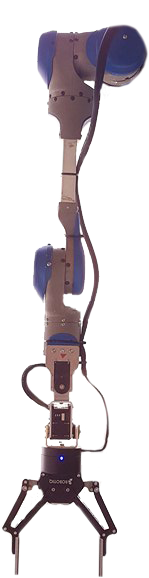
\includegraphics[width=0.10\textwidth]{images/arm.png}
	\caption{Bras à 7 degrés de liberté}
\end{wrapfigure}

L'autre aspect principal qui fut amélioré était la base de notre robot. Suite à notre première compétition en Allemagne, nous avons observé que la base était beaucoup trop large, ce qui causait quelques problèmes au niveau de la navigation autonome près des portes. En se basant sur ces observations, nous décidé de réduire la largeur, ce qui a eu pour effet d'améliorer grandement les capacités en navigation. \\
\newpage
\section{Logiciel}

\subsection{Planification des tâches de haut-niveau}
Afin de planifier l'ensemble des tâches que notre plateforme pouvait accomplir, nous avons utilisé un module développé par une équipe de robotique participant à la compétition Darpa Robotics Challenge. Ce logiciel nommé \href{http://philserver.bplaced.net/fbe/index.php}{FlexBe}\cite{schillinger2016flexbe}, pour Flexible Bahavior, est composé d'une interface de style programmation par blocs, il est donc facile et clair d'implémenter les différents scénarios pour la compétition.\\


\begin{figure}[h!]
	\centering
	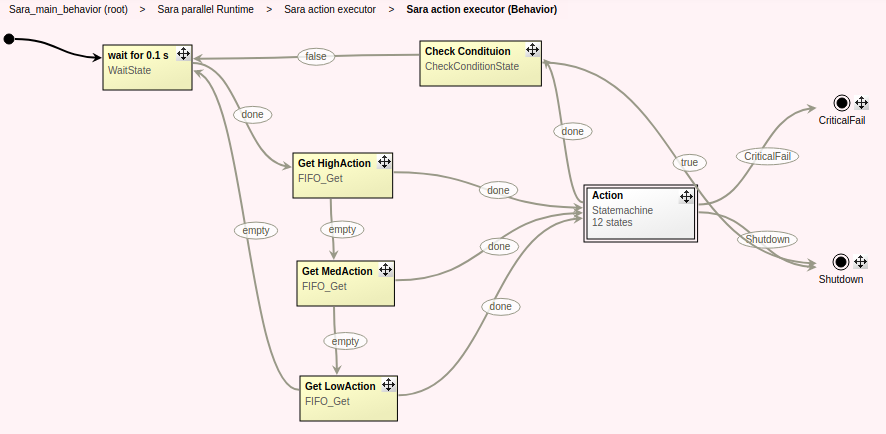
\includegraphics[width=0.70\textwidth]{images/flexbe.png}
	\caption{Représentation de FlexBe}
\end{figure}

Par contre, nous n'utilisons pas tout simplement FlexBe, nous devons programmer nos propres états en utilisant l'API en python. Pour simplifier notre travail, nous avons commencé par diviser tous les scénarios de base demandés lors de la compétition Robocup@Home en petites actions reproductibles. Nous avons ensuite repéré ceux pouvant être accomplis par notre robot et les avons transformés en état (ex : mouvement du bras à une position X). Ces blocs d'état peuvent ensuite être assemblés ensemble pour former une hiérachie plus élevée que l'on nomme Actions. Nous assemblons finalement ces actions en ActionWrapper qui permettront d'interfacer les actions générales de notre robot avec la détection vocale ainsi que le traitement du langage. Ces différents modules interprètent ainsi le langage et le transforment en actions réalisables par le robot. Cette structure récursive nous permet donc un développement beaucoup plus rapide pour chaque tâche nécessaire. \\

\subsection{Traitement du langage naturel}

Pour analyser les commandes vocales détectées, nous nous appuyons sur un logiciel développé par le \href{http://sag.art.uniroma2.it/}{Groupe d'analyse sémantique de l'Université de Roma} et le \href{http://labrococo.dis.uniroma1.it /}{Laboratoire de robots coopératifs cognitifs} à l'Université Sapienza de Rome. Cet analyseur vocal, appelé \href{http://sag.art.uniroma2.it/lu4r.html}{LU4R} \cite{lu4r} pour "Language Understanding For Robots", est composé d'un serveur développé en Java qui prend en entrée, la phrase détectée et l'environnement sémantique entourant le robot. \\

Ce serveur communique via un service REST qui lui donne la possibilité d'être compatible avec tout type de plateforme. Tout ce qui doit être fait, c'est de lancer le serveur localement qui est compilé à travers un fichier .jar. Encore une fois, cela donne l'opportunité d'utiliser ce logiciel sur toutes les plateformes, que vous utilisiez Windows, Linux ou Mac. Ce logiciel donne la possibilité d'obtenir différentes représentations en sortie. Nous avons choisi la \href{https://github.com/amrisi/amr-guidelines/blob/master/amr.md}{représentation amr} car c'était la plus facile à comprendre et à mettre en œuvre. \\

Nous avons décidé de créer notre propre wrapper ROS, \href{https://github.com/WalkingMachine/lu4r_ros}{lu4r\_ros} pour mieux l'intégrer à notre approche de planification des tâches. Nous traduisons d'abord la réponse donnée par LU4R au format simple, que nous appelons ActionForms. Un ActionForms contient une action suivie de tous ses paramètres possibles identifiés dans l' \href{https://framenet2.icsi.berkeley.edu/fnReports/data/luIndex.xml}{Index FrameNet des unités lexicales}. Les ActionWrappers sont ensuite introduits dans un gestionnaire de priorités FIFO et finalement envoyés à notre planificateur de tâches. \\

Ce qui est également intéressant à propos de LU4R, c'est qu'il utilisera la cartographie sémantique dans son processus d'analyse. Pour cela, nous devons fournir la pose exacte pour chaque objet dans l'environnement du robot. Il est également possible de préciser divers synonymes pour chaque objet afin de mieux comprendre la phrase en entrée. \\


\subsection{Reconnaissance d'objets}

En tant qu'équipe débutante, nous explorons encore diverses solutions autour du problème de la reconnaissance d'objets. Notre première approche était d'utiliser le paquet ROS ORK (object recognition kitchen) de Willow Garage. Mais, après l'avoir utilisé en compétition, nous avons réalisé que la performance et la facilité d'utilisation n'étaient pas l'approche que nous recherchions. Comme alternative, nous avons commencé à utiliser le paquet YOLO \cite{yolo} (You Only Look Once). \\

YOLO permet la détection d'objets en temps réel. Il ne détecte pas seulement divers objets, mais il prédit également la boîte de délimitation de l'objet détecté. Il utilise un réseau de neurones qui est appliqué à l'image. Plusieurs régions sont ensuite créées et sont utilisées pour prédire les zones de délimitation. Chaque objet contient également son niveau de confiance indiquant à quel niveau nous sommes certains du type d'objet détecté, qui est ensuite utilisé pour filtrer ces derniers. L'avantage de ce système est qu'il peut détecter plusieurs objets en même temps dans un scénario temps-réel. \\

 
\begin{figure}
  \centering
  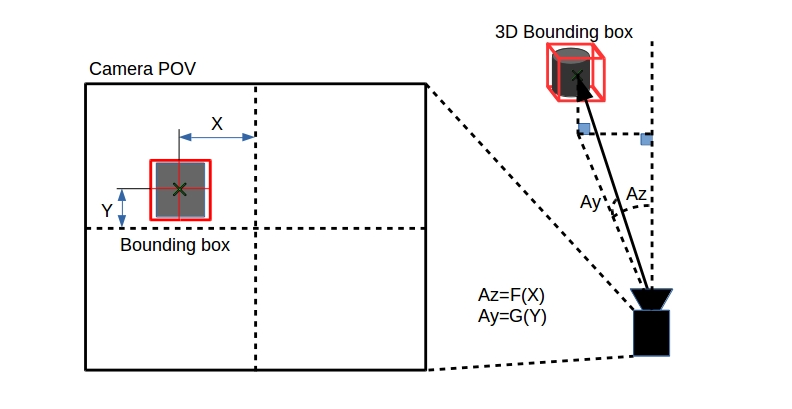
\includegraphics[width=200pt]{images/frame_to_box.png}
  \caption{Boîte de délimitation 2D vers la pose de préhension en 3D, technique actuelle}
\end{figure} 
 
Nous utilisons le paquet ROS pour faciliter notre travail, car cela nous permet d'obtenir directement la sortie des objets reconnus dans un "topic" ROS. Nous pouvons également obtenir la boîte de délimitation pour chaque objet détecté. La première étape que nous avons dû faire était de transformer ces boîtes 2D en 3D afin d'obtenir une pose relative à notre robot. \\

Pour le moment, nous avons créé le paquet \href{https://github.com/WalkingMachine/wm_frame_to_box}{wm\_frame\_to\_box} pour approcher la pose de l'objet utilisant le pixel de profondeur se retrouvant au centre de la boîte. Même si elle peut présenter des failles, cette technique s'est également avérée largement suffisante pour la plupart de nos applications et, plus importante encore, elle utilise beaucoup moins de puissance de traitement que la correspondance de formes 3D utilisée auparavant. Cela nous permet de faire du positionnement d'objets en temps réel, une fonctionnalité dont nous sommes fiers d'avoir accompli. \\

Par la suite, pour obtenir de meilleurs résultats et une meilleure pose, nous prévoyons soustraire le nuage de points en fonction des limites. Nous l'utiliserons ensuite avec la segmentation de nuage de points de la bibliothèque \href{http://pointclouds.org}{PCL} pour extraire l'objet spécifique et l'envoyer à un paquet d'identification de saisie comme \href{http://wiki.ros.org/haf_grasping}{haf\_grasping}. Cette technique, comparée à ce que nous utilisons actuellement, nous donnerait la possibilité de saisir une plus grande variété d'objets. \\

\begin{figure}
  \centering
  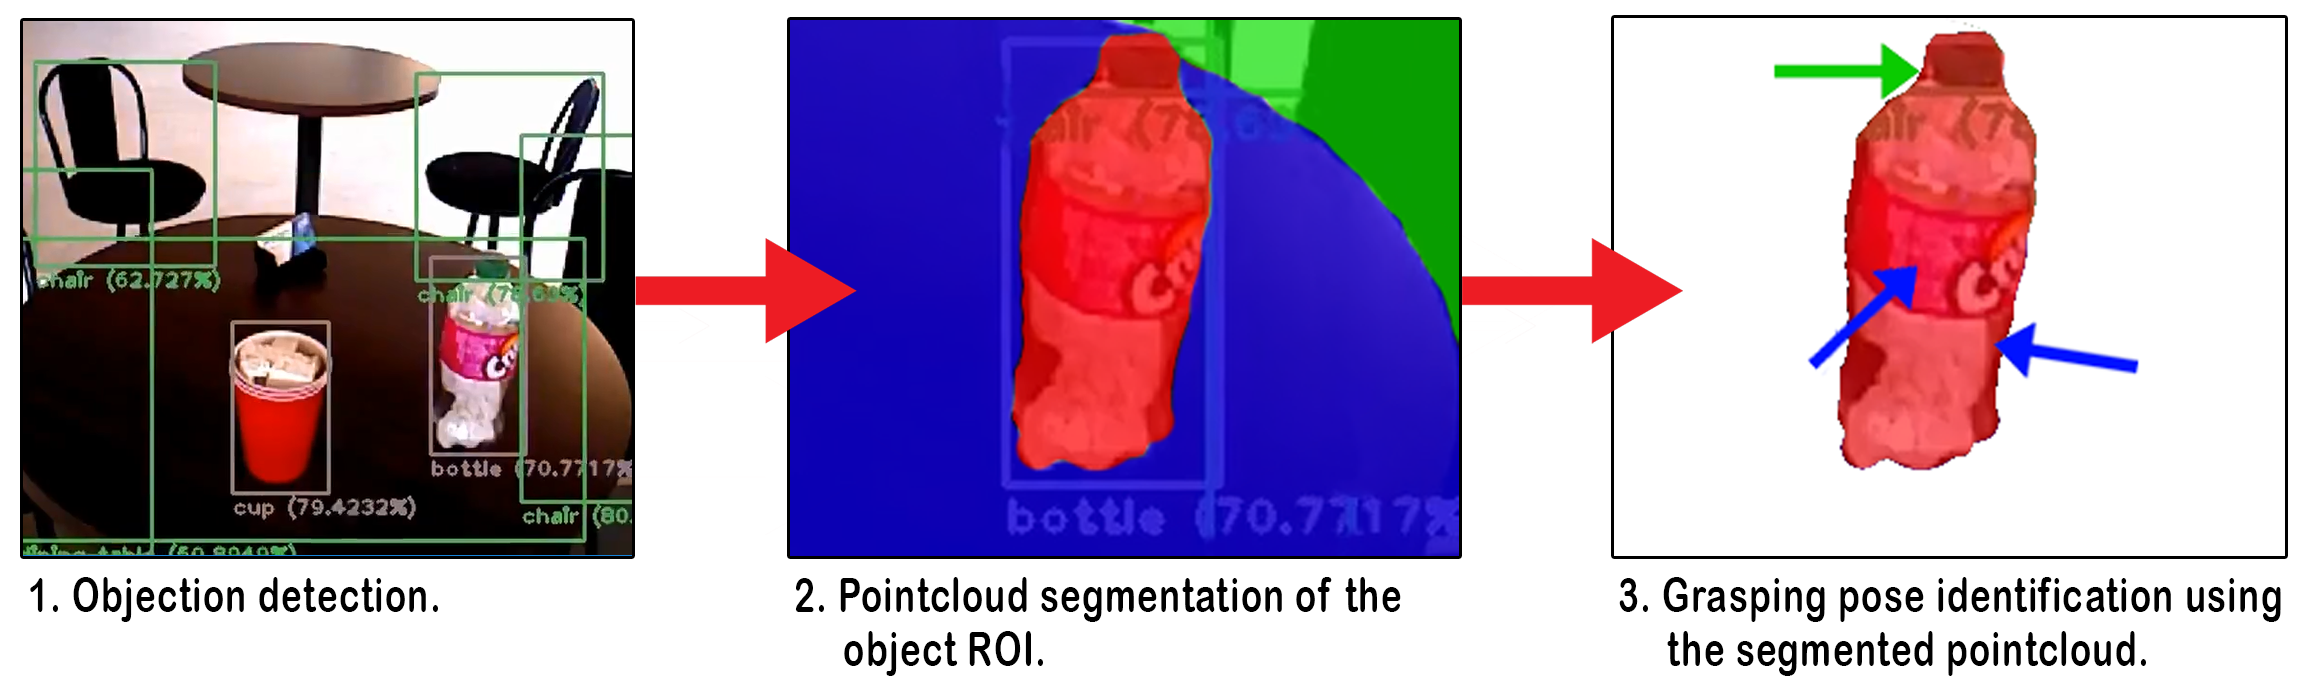
\includegraphics[width=300pt]{images/frame_to_box2.png}
  \caption{Boîte de délimitation 2D vers la pose de préhension en 3D, technique future}
\end{figure}

Pour l'instant, nous utilisons le modèle YOLO, mais nous souhaitons entrainer notre proposer ensemble de données, comme nous le ferions en compétition. C'est nouveau pour nous, mais, nous avons tous les outils dont nous avons besoin pour surmonter cela. \\

\subsection{Navigation}
En plus de notre système de navigation précédemment utilisé, cette année nous utilisons le module \href{http://wiki.ros.org/pointcloud_to_laserscan}{pointcloud\_to\_lasercan} comme solution plus légère afin de faire de l'évitement d'objets en 3D. Cela nous assure une navigation beaucoup plus sécuritaire puisqu'en utilisant seulement une navigation 2D à l'aide d'un lidar, il serait possible que le robot entre en collision avec une table puisqu'il ne verrait que les pattes de celle-ci. Un autre avantage de cette implémentation est qu'il est possible de spécifier la hauteur maximum au niveau des collisions. Ainsi, nous évitons également les possibles collisions avec la tête de notre robot. \\

\subsection{Représentation de l'environnement}
Comme nouveauté cette année, nous avons implémenté notre propre solution afin de représenter l'environnement entourant le robot d'une façon simple pour tout le monde. Notre solution que nous avons nommée \href{http://github.com/walkingmachine/wonderland}{wonderland} est un système agnostique dans le même genre que LU4R présenté plus tôt. Elle est composée d'un serveur recevant une requête HTTP basée sur un API développé par l'équipe.\\

La première chose requise pour commencer à utiliser cette plateforme, est l'action de populer la base de données. Cela peut être fait de façon manuelle en indiquant la position de chaque objet connu, mais cela peut être fait par le robot à l'aide de requête POST. Il est également possible de spécifier une pièce avec une position relative à celle-ci. Lorsque les différentes informations sont insérées, il est possible de faire une requête GET sur l'adresse définissant le serveur de wonderland (ex : http://wonderland:8000/object). Cette dernière retournera la liste complète des objets contenus dans la base de données. Il est également possible de filtrer les demandes en rajoutant par exemple une couleur ou une position comme paramètre. \\

Puisque la base de données est hébergée sur un serveur, il est possible d'y accéder depuis n'importe où. Il est possible de l'exporter sur un autre ordinateur, de la mettre en infonuagique ou seulement de l'installer sur l'ordinateur même du robot. Cela donne également la possibilité d'avoir une connaissance dynamique, ce qui signifie que le robot peut mettre à jour ses connaissances de l'environnement en temps réel.\\



\section{Conclusion et projets futurs} 
Comme vous pouvez le constater, malgré que nous soyons une équipe composée principalement d'étudiants de premier cycle, nous sommes tout de même capables de rivaliser avec les autres équipes issues de laboratoire de recherche. Nous avons récemment mis beaucoup d'efforts afin d'avoir une plateforme plus stable et de réduire les différents problèmes présents, nous permettant donc d'avancer dans la bonne direction. \\

Avec notre nouveau système de batteries interchangeables, notre détection d'objets et l'interprétation du langage naturel, notre robot est devenu une plateforme autonome complètement fonctionnelle, nous permettant ainsi de nous concentrer sur le coeur des défis de la compétition.\\

\section*{Robot SARA Hardware Description}
% TODO Change picture and description
Specifications for robot SARA are as follows:

\begin{table}

\label{my-label}

\begin{tabular}{l|p{90mm}}
\hline
\rowcolor[HTML]{FFFFFF} 
\multicolumn{2}{c}{\cellcolor[HTML]{FFFFFF}\textbf{SARA}}                                                      \\ \hline
\rowcolor[HTML]{EAEFF6} 
\textbf{Base}               & Custom base with fully holonomic platform                                        \\
\rowcolor[HTML]{FFFFFF} 
\textbf{Right arm}          & 7 DoF custom arm made of Kinova motors                                           \\
\rowcolor[HTML]{EAEFF6} 
\textbf{Neck}               & Tilt and pan unit using two Dynamixel MX-64R servo actuator                      \\
\rowcolor[HTML]{FFFFFF} 
\textbf{Head}               & Custom head made of RGB neopixels leds and Asus Xtion Pro                        \\
\rowcolor[HTML]{EAEFF6} 
\textbf{Gripper}            & Robotiq 2 fingers 140mm                                                           \\
\rowcolor[HTML]{FFFFFF}
\textbf{Dimensions}         & \begin{tabular}[c]{@{}l@{}}Base : 0,61m. X 0,77m.\\ Height : 1,68m.\end{tabular} \\
\rowcolor[HTML]{EAEFF6} 
\textbf{Weight}             & $\sim$60kg                                                                      \\
\rowcolor[HTML]{FFFFFF} 
\textbf{Additional sensors} & Hokuyo UTM-30LX on base                                                          \\
\rowcolor[HTML]{EAEFF6} 
\textbf{Microphone}         & Rode microphone											                         \\
\rowcolor[HTML]{FFFFFF} 
\textbf{Batteries}          & 2x 20V Dewalt drill battery 5aH                                                 \\
\rowcolor[HTML]{EAEFF6} 
\textbf{Computer}           & 1x Lenovo p50 with 32GB RAM and nVidia Quadro M2000 4GB, 1x Raspberry Pi 3       \\ \hline
\end{tabular}
\caption{Robot's hardware description}
\end{table}
\begin{wrapfigure}[10]{r}{0.25\textwidth}
	\centering
	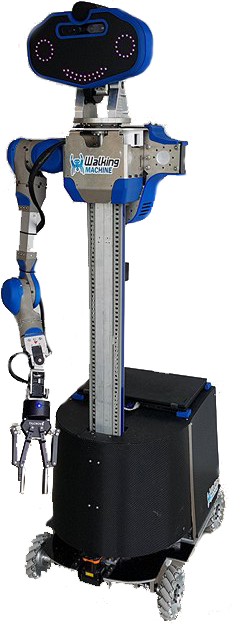
\includegraphics[width=0.30\textwidth]{images/sara_2.png}
	\caption{Robot SARA}
\end{wrapfigure}
\section*{Robot's Software Description}

For our robot we are using the following software:

\begin{itemize}
	\item Platform: Robotic Operating System (ROS) Kinetic on Ubuntu 16.04
	\item Navigation, localization and mapping: \href{http://wiki.ros.org/gmapping}{Gmapping}, \href{http://wiki.ros.org/amcl}{AMCL}, \href{http://wiki.ros.org/pointcloud_to_laserscan}{pointcloud\_to\_laserscan}
	\item Face recognition: \href{http://wiki.ros.org/people}{People}
	\item Speech recognition: \href{https://github.com/WalkingMachine/lab_ros_speech_to_text}{Google Speech API}
	\item Speech comprehension: \href{http://sag.art.uniroma2.it/lu4r.html}{LU4R}, \href{https://github.com/WalkingMachine/lu4r_ros}{lu4r\_ros}
	\item Speech generation: \href{https://doc.ubuntu-fr.org/svoxpico}{Svoxpico}
	\item Object recognition: \href{https://github.com/WalkingMachine/wm_darknet}{Darknet with YOLO v2 }
	\item Arm control: \href{http://wiki.ros.org/moveit}{MoveIt} and \href{https://github.com/Kinovarobotics/kinova-ros}{Kinova API}
	\item Task executor: \href{http://wiki.ros.org/flexbe}{Flexbe} 
	\item World reprensentation: \href{http://github.com/walkingmachine/wonderland}{Wonderland}
\end{itemize}
	

\section*{Membres de l'équipe}
Jeffrey Cousineau, Philippe La Madeleine, Maxime St-Pierre, Nathalie Connolly, Jimmy Poirier, Léonore Jean-François, Samuel Otis, Redouane Laref, Louis-Charle Labarre, Lucas Maurice, Nicolas Nadeau, Simon Landry, Cheuk Fai Shum, Veronica Romero Rosales, Nicolas Bernatchez, Quentin Gaillot, Raphael Duchaine, Jean-Frederic Boivin 

\nocite{*}
\bibliographystyle{plain}
\bibliography{references}


\end{document} 
